% !TEX program = xelatex
\documentclass[addpoints,11pt]{exam}
\usepackage{fontspec}
\usepackage[T1]{fontenc} % uses T1 fonts (better quality)
\usepackage{lmodern} % uses Latin Modern fonts
% \usepackage[margin=1in]{geometry} % not needed with exam class
\usepackage[dvipsnames]{xcolor}
% \usepackage{ragged2e}
% \renewcommand{\baselinestretch}{1.15}
\usepackage{tikz}
\usetikzlibrary{automata,scopes,shapes,matrix,arrows,decorations.pathmorphing}
\tikzset{>={stealth}}
\usepackage{amsmath,amsfonts,amssymb}
\usepackage{bm}

\usepackage{graphicx}
\graphicspath{ {./graphics/} }
\usepackage{tcolorbox}
\usepackage{etoolbox}
\usepackage[dvipsnames]{xcolor}
\definecolor{CrispBlue}{HTML}{0176AE}

\usepackage[makeroom]{cancel}
\definecolor{OuterBlue}{HTML}{1370AA}
\definecolor{InnerBlue}{HTML}{9BC4DD}
\usepackage{pdfpages}

\BeforeBeginEnvironment{verbatim}{\footnotesize}%
\AfterEndEnvironment{verbatim}{\textnormal}%

\begin{document}
% \setmainfont{SF Pro Text}
% \setsansfont{SF Pro Text}
\setmonofont{SF Mono}
% \renewcommand{\familydefault}{\sfdefault}

\begin{center}
    % \line(1,0){300}\\[0.25cm]
 	\large\bfseries ECE 538 - Advanced Computer Architecture\\
    Homework Assignment 2 (Individual)\\[1em]
    100 points\\[1em]
    Assigned Date: \textnormal{10/11/2021} Due Date: \textnormal{10/21/2021}\\[5em]
    David Kirby \quad davidkirby@unm.edu
 	% \line(1,0){300}\\[0.75cm]
    % \textnormal{
    % \cvpword{Credits}\cvbpword{Extra Credits}
    % \combinedgradetable[v][questions]}
    \end{center}
    \pagestyle{headandfoot}
    \firstpagefooter{}{\thepage}{}
    \runningfooter{}{\thepage}{}
    \newpage

\begin{questions}
    \pointformat{(\thepoints)}
    \pointpoints{point}{points}
    \bonuspointformat{(\thepoints)}
    \bonuspointpoints{extra credit}{extra credits}

\question\textbf{(\pointsofquestion{1} points)} % Question 1
    Answer the following qualitative questions:
    \begin{parts}
        \part[5] What are the types of cache misses discussed in lecture so far? Briefly describe each.

        \begin{tcolorbox}[colback=CrispBlue!5!white,colframe=CrispBlue!75!black,title=]
            \begin{enumerate}
                \item Compulsory: These are the initial misses due to an empty (cold) cache.
                \item Conflict: These are the misses due to a rigid block placement strategy (i.e. low associativity).
                \item Capacity: These are misses due to the cache being too small to hold the entire working set of data and instructions.
            \end{enumerate}
        \end{tcolorbox}
        \vspace{\stretch{1}}

        \part[5] How can pipelining the L1 cache improve processor performance? What negative effects can it have?

        \begin{tcolorbox}[colback=CrispBlue!5!white,colframe=CrispBlue!75!black,title=]
            Pipelining the L1 cache increases the cache bandwidth, but negatively affects the hit time.
        \end{tcolorbox}
        \vspace{\stretch{1}}

        \part[5] How does a direct-mapped cache compare to a set-associative cache in terms of access time, logic complexity, energy, etc.?
        
        \begin{tcolorbox}[colback=CrispBlue!5!white,colframe=CrispBlue!75!black,title=]
            Associativity reduces conflict misses by providing a more flexible block placement strategy. For example, direct-mapped has only one location in the cache that a block can be placed, but full-associativity allows blocks to be placed anywhere in the cache.\vspace{1em}

            While a set-associative cache decreases the miss rate, the drawbacks to associativity include increased complexity, access (hit) time, and power as well as added difficulty when pipelining the cache.
        \end{tcolorbox}
        \vspace{\stretch{1}}

        \part[5] What is Average Memory-Access Time (AMAT)? And how it can be calculated?

        \begin{tcolorbox}[colback=CrispBlue!5!white,colframe=CrispBlue!75!black,title=]
            Average memory-access time is an indirect measure of cache performance; although it is a better measure than miss rate, it is not a substitute for execution time.
            \begin{align}
                \notag\text{AMAT} = \text{hit time} + \text{miss rate} \times \text{miss penalty}
            \end{align}
        \end{tcolorbox}
        \vspace{\stretch{1}}
    \end{parts} 
\newpage 

\question\textbf{(\pointsofquestion{2} points)} % Question 2
Assume you have an \textit{in-order} RISC processor that has a CPI of 1.3 with an ideal memory hierarchy (i.e., all memory accesses hit in the L1 caches). For a given benchmark, 38\% of instructions executed are loads and stores. The miss penalty for reads and writes to the L1 data cache is 20 clock cycles and the miss rate is 3\%.
    \begin{parts}
        \part[5] Calculate the CPI of your RISC processor taking memory stalls due to data accesses into account.
        
        \begin{tcolorbox}[colback=CrispBlue!5!white,colframe=CrispBlue!75!black,title=]\vspace{-1em}
            \begin{align}
                \notag\text{CPI} &= \frac{\text{clock cycles}}{\text{instruction}} + \text{miss rate} \times \text{miss penalty}\\
                \notag &= 1.3 + 0.38 \times 0.03 \times 20\\
                \notag &= 1.528\ \frac{\text{clock cycles}}{\text{instruction}}
            \end{align}
        \end{tcolorbox}
        \vspace{\stretch{1}}
    
        \part[5] The miss penalty for the L1 instruction cache is also 20 clock cycles and the miss rate is 1\%. Recalculate the CPI of your processor taking into account stalls from both the instruction and data caches. How much faster is the machine with the ideal memory system?
        
        \begin{tcolorbox}[colback=CrispBlue!5!white,colframe=CrispBlue!75!black,title=]\vspace{-1em}
            \begin{align*}
                \text{CPI} &= \frac{\text{clock cycles}}{\text{instruction}} + \text{miss rate} \times \text{miss penalty}\\
                &= 1.3 + 0.01 \times 20 + 0.38 \times 0.03 \times 20\\
                &= 1.728\ \frac{\text{clock cycles}}{\text{instruction}}\\[1em]
                \text{Speedup} &= \frac{\text{CPI}_\text{stalls}}{\text{CPI}_\text{ideal}}\\
                &= \frac{1.728}{1.3}\\
                &=1.329 \times
            \end{align*}
        \end{tcolorbox}
        \vspace{\stretch{1}}

        \part[5] Assuming your processor runs at 1 GHz, what is the average memory access time of the L1 instruction cache? What is the average memory access time of the L1 data cache?
        
        \begin{tcolorbox}[colback=CrispBlue!5!white,colframe=CrispBlue!75!black,title=]\vspace{-1em}
            \begin{align*}
                \text{1 GHz} = \text{1 ns}/ \text{clock cycle}, \hspace{3em}
                \text{AMAT} &= \text{hit time} + \text{miss rate} \times \text{miss penalty}\\[1em]
                \text{AMAT}_I &= 1\text{ ns}+0.01\times 20\text{ ns}\\
                &= 1.2\text{ ns}\\
                \text{AMAT}_D &= 1\text{ ns}+0.03\times 20\text{ ns}\\
                &= 1.6\text{ ns}
            \end{align*}
        \end{tcolorbox}
        \vspace{\stretch{1}}

        \part[5] Why might the hit rate be higher for the instruction cache compared to the data cache?
        
        \begin{tcolorbox}[colback=CrispBlue!5!white,colframe=CrispBlue!75!black,title=]
            Instruction cache exhibits a lot more spatial and temporal locality compared to data access cache.
        \end{tcolorbox}
        \vspace{\stretch{0.1}}

        \part[5] Calculate the \textit{misses per instruction} for both instruction and data caches. How does this metric differ from \textit{miss rate}?

        \begin{tcolorbox}[colback=CrispBlue!5!white,colframe=CrispBlue!75!black,title=]\vspace{-1em}
            \begin{align*}
                \frac{\text{Misses}}{\text{Instruction}} &= \text{Miss rate} \times \frac{\text{Memory accesses}}{\text{Instruction}}\\[1em]
                \frac{\text{Misses}}{\text{Instruction}}(I) &=0.01 \times 1\\
                &=0.01\\
                \frac{\text{Misses}}{\text{Instruction}}(D) &=0.03 \times (1+0.38)\\
                &=0.0138
            \end{align*}
            This metric differs (as is shown in the equation above) by accounting for the memory accesses per instruction. In this example, 38\% of our instructions access memory (in the form of data reads and writes); therefore, we see a higher miss per instruction.
        \end{tcolorbox}
        \vspace{\stretch{1}}
    \end{parts}
\newpage

\question\textbf{(\pointsofquestion{3} points)} % Question 3
You are designing a System On a Chip (SoC) with your 5-stage pipelined RISC processor. The minimum system requirements are 512KB of program ROM and 16KB of RAM. For a given technology node, the critical path of your processor (ignoring memory access) is 1 ns. The access time for a 512KB ROM in the same technology is 2.0 ns, while the access time for a 16KB RAM is 0.8 ns.
    \begin{parts}
        \part[5] Assuming the Fetch and Memory stages of your processor only access memory and the flip-flop overhead is 0.1 ns, what is the fastest achievable clock rate of your processor when directly fetching instructions from the program ROM?
        
        \begin{tcolorbox}[colback=CrispBlue!5!white,colframe=CrispBlue!75!black,title=]
            \begin{align*}
                \text{Clock rate} &= \frac{1}{\text{ROM access time} + \text{overhead}}\\
                &= \frac{1}{2\text{ ns} + 0.1 \text{ ns}}\\
                &= 476 \text{ MHz}
            \end{align*}
        \end{tcolorbox}
        \vspace{\stretch{1}}

        \part[5] Assuming accesses to program ROM are cached in a 4KB instruction cache with an access time of 0.5 ns, what is the fastest achievable clock rate of your processor?

        \begin{tcolorbox}[colback=CrispBlue!5!white,colframe=CrispBlue!75!black,title=]
            Since the access time for the instruction cache is less than the critical path of the processor (i.e., 0.5 ns < 1 ns), the processor will actually be the bottleneck in this scenario; therefore, the fastest achievable clock rate would be 1 GHz.
        \end{tcolorbox}
        \vspace{\stretch{1}}

        \part[10] If the miss rate of the 4KB instruction cache with a 16 byte block size is 6.3\% for a given workload, what is the average number of memory stall cycles per instruction your processor will see with a 4KB instruction cache? Assume the instruction cache can start a read from program ROM on the cycle after the miss is detected, and critical word first is not implemented.

        \textit{Hint:} Start by calculating the miss penalty in clock cycles and remember a cache miss fills an entire line.

        \begin{tcolorbox}[colback=CrispBlue!5!white,colframe=CrispBlue!75!black,title=]
            \begin{align*}
                \text{Miss penalty} &= 1^{\text{st}}\text{ cycle to detect miss} + \text{\# to fill cache} \times \text{cycles to read ROM}\\
                &= 1\text{ cycles} + 1 \times (0.5 + 0.1) \text{ cycles}\\
                &= 1.6 \text{ cycles}
            \end{align*}
            \begin{align*}
                \frac{\text{Memory stall cycles}}{\text{Instruction}} &= \text{Instruction count} \times \text{Miss rate} \times \text{Miss penalty}\\
                &= 1 \times 0.063 \times 1.6 \text{ cycles}\\
                &\approx 1 \text{ cycle}
            \end{align*}
        \end{tcolorbox}
        \vspace{\stretch{1}}

        \part[10] Without the instruction cache, the processor is able to complete 4 million instructions from the same workload in 4.8 million clock cycles. What will be the CPI of your processor with the 4KB instruction cache, assuming the same workload?
        
        \begin{tcolorbox}[colback=CrispBlue!5!white,colframe=CrispBlue!75!black,title=]
            \begin{align*}
                \text{CPI}_{\text{initial}} &= \frac{4.8\text{ million cycles}}{4 \text{ million instructions}}\\
                &= 1.2\ \frac{\text{cycles}}{\text{instruction}}\\[1em]
                \text{Memory stall cycles}_{\text{cache}} &= \text{Instruction count} \times \text{Miss rate} \times \text{Miss penalty}\\
                &= 4\text{ million} \times 0.063 \times 1 \text{ cycles}\\
                &= 252,000 \text{ cycles}\\[1em]
                \text{Cycles}_{\text{total}} &= 4.8 \text{ million} + 252,000\\
                &= 5.052 \text{ million cycles}\\[1em]
                \text{CPI}_{\text{cached}} &= \frac{\text{stalled}}{\text{ideal}}\\
                &= 1.263\ \frac{\text{clock cycles}}{\text{instruction}}
            \end{align*}
        \end{tcolorbox}
        \vspace{\stretch{1}}
    \end{parts}
\newpage

\question\textbf{(\pointsofquestion{4} points)} % Question 4
Consider the following simple C code for matrix transpose:
\begin{verbatim}
    for (i = 0; i < 1024; i++){
        for (j = 0; j < 1024; j++){
            Y[j][i] = X[i][j]
        }
    }
\end{verbatim}
\normalsize
Assume that both \texttt{X} and \texttt{Y} are stored in the row major order and each element in the matrices is a double word (64-bit) integer.
    \begin{parts}
        \part[5] Execute the code on your laptop and report the execution time. Would loop interchange help improve the performance of the code? Give explanation.

        \begin{tcolorbox}[colback=CrispBlue!5!white,colframe=CrispBlue!75!black,title=]
            Transpose using the base code took 14.690 milliseconds to execute. Interchanging the loops certainly helps by increasing the locality of the data. When an array is loaded into cache from memory, it loads the entire block, meaning the next call will only have to go to cache, and not memory. When using loop exchange, the transpose took 10.229 milliseconds to execute, which equates to a 1.436\( \times \) speedup.
        \end{tcolorbox}
        \vspace{\stretch{1}}

        \part[10] Rewrite the code by applying blocking (the software technique to improve data reuse). Use a blocking factor that leads to a noticeable performance improvement on the same computer as the one used in (a). Explain your reason for choosing the specific blocking factor.

        \begin{tcolorbox}[colback=CrispBlue!5!white,colframe=CrispBlue!75!black,title=]
            The main purpose of loop-blocking is to eliminate as many cache misses as possible by breaking up the memory into smaller chunks. In this case I chose to break it up into 8-bit chunks, and then transposed from there.
        \end{tcolorbox}
        \vspace{\stretch{1}}

        \part[10] Execute the new code and report the execution time. Make a comparison with the results reported in (a).
        \begin{tcolorbox}[colback=CrispBlue!5!white,colframe=CrispBlue!75!black,title=]
            Loop-blocking resulted in a transpose time of 8.697 milliseconds, which compared to our results in (a) equates to a 1.689\( \times \) speedup over the base code and a 1.176\( \times \) speedup over the interchanged code. See figure below for outputs.
        \end{tcolorbox}
        \begin{figure}[ht]
            \centering
            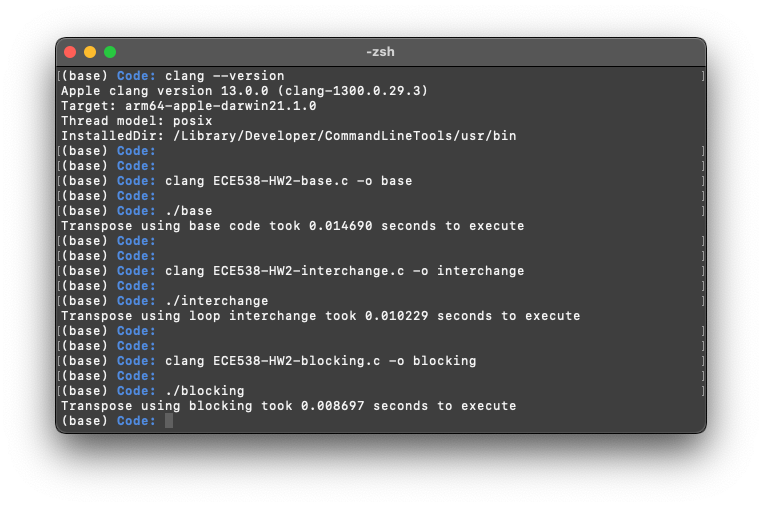
\includegraphics[width=\linewidth]{timeTrials.png}
            % \caption{Time trials of transposes.}
            % \label{fig:timeTrials}
        \end{figure}

        \vspace{\stretch{1}}
    \end{parts}
\end{questions}
\end{document}
